\documentclass[runningheads,oribibl]{llncs}

\usepackage{graphicx}
\graphicspath{{./figures/}{./}}
\usepackage{amsmath}
\usepackage{amssymb}
\usepackage{booktabs}
\usepackage{array}
\usepackage[protrusion=true,expansion=false]{microtype}
\usepackage[colorlinks=true, linkcolor=blue, citecolor=blue, urlcolor=blue]{hyperref}

\setlength{\textfloatsep}{10pt plus 2.0pt minus 2.0pt}
\setlength{\floatsep}{8pt plus 2.0pt minus 2.0pt}
\setlength{\intextsep}{8pt plus 2.0pt minus 2.0pt}

\begin{document}

\title{Empirical Evaluation of Activation-Aware Weight Quantization for Edge LLM Inference on Unified Memory Architectures}
\titlerunning{Activation-Aware Quantization on Unified Memory}

\author{Neeraj Kumar\inst{1}\orcidID{0009-0006-6997-3283} \and
Sowmya Pidathala\inst{1} \and
Uday Panwar\inst{2}}
\authorrunning{N. Kumar et al.}

\institute{Department of Artificial Intelligence, Indian Institute of Information Technology Vadodara - ICD, India\\
\email{\{20262603008, 20262603011\}@iiitvadodara.ac.in}
\and
Department of Electronics and Communication Engineering, Indian Institute of Information Technology Vadodara - ICD, India\\
\email{uday\_panwar@iiitvadodara.ac.in}}

\maketitle

\begin{abstract}
On-device inference with autoregressive language models runs into a hard physical constraint: DRAM bus saturation during single-sequence generation. At batch size $B=1$, the hardware must stream every parameter from main memory for each generated token. Operating in 16-bit floating point keeps operational intensity stalled near 1.0 FLOP per byte, leaving local GPU cores idle while waiting on bus transfers. Post-training 4-bit integer quantization ($W4A16$) cuts parameter bandwidth by nearly three quarters, yet uniform round-to-nearest (RTN) methods introduce severe distortion because a small subset of channels develop extreme activation magnitudes. In this paper, we evaluate Activation-aware Weight Quantization (AWQ) on an Apple M1 system using unified memory architecture (UMA). Profiling real weights and activations from \texttt{TinyLlama-1.1B}, we show that activation kurtosis is sharpest in early self-attention projections (\texttt{v\_proj} and \texttt{q\_proj}), where outlier spikes reach $206.42\times$ the channel average. Pre-quantization scale rebalancing drops reconstruction error on these layers by up to $91.91\%$ ($+10.92$~dB SNR) relative to standard RTN. From a systems perspective, setting group size $G=128$ yields 64-byte payload blocks that map into Apple Silicon's 128-byte cache lines at two groups per line (assuming decoupled scale storage), preventing split-line DRAM fetches while reducing total weight movement across the memory bus by $74.2\%$, which projects an estimated $3.88\times$ theoretical latency speedup under memory-bound decoding.

\keywords{Edge AI \and Post-Training Quantization \and Unified Memory \and Memory Bandwidth \and Apple Silicon \and TinyLlama.}
\end{abstract}

\section{Introduction}
Cloud-centric serving frameworks optimize for throughput by bundling concurrent queries into large batches ($B \ge 64$)~\cite{sheng2023flexgen}. This strategy reuses loaded model parameters across multiple tokens, keeping matrix units fed at high arithmetic intensities.

Edge execution operates under entirely different constraints. On personal workstations or laptops running local interactive models, batch sizes remain strictly single-user ($B=1$). Under these conditions, the execution profile is dominated by parameter transfers rather than compute. For an $M$-parameter model stored in FP16, producing a single token requires executing $2M$ floating-point operations while pulling $2M$ bytes across the DRAM bus. The operational intensity - defined under the Roofline model~\cite{williams2009roofline} as the ratio of floating-point computations performed per byte transferred from memory - caps out at 1.0 FLOP/byte.

We evaluate this behavior on a stock Apple MacBook Air M1 (8-core CPU, 7-core GPU, unified LPDDR4X memory with 68.25 GB/s peak bandwidth)~\cite{apple2020m1}. In this Unified Memory Architecture (UMA), CPU cores, GPU execution pipelines, and neural accelerators access a single shared DRAM pool without discrete PCIe bus transfer bottlenecks. Streaming \texttt{TinyLlama-1.1B} (2.2 GB in FP16) saturates the memory bus and limits decoding to roughly 25--30 tokens per second. Although the integrated GPU is capable of 2.6 TFLOPs (trillion floating-point operations per second) of half-precision throughput, compute pipelines remain stalled on memory transactions during more than $95\%$ of each step. The bottleneck is memory bandwidth.

Post-training quantization to 4-bit weights ($W4A16$) directly mitigates this bus traffic~\cite{frantar2022gptq,dettmers2023qlora}. Yet uniform round-to-nearest (RTN) rounding introduces heavy distortion. Transformer hidden states exhibit severe channel kurtosis: fewer than $1\%$ of channels produce activation magnitudes multiple orders of magnitude higher than the median~\cite{dettmers2022llmint8,xiao2023smoothquant}. When weights paired with these outlier channels undergo uniform integer rounding, the resulting quantization noise spreads through subsequent layers.

Activation-aware Weight Quantization (AWQ)~\cite{lin2024awq} avoids irregular mixed-precision formats by scaling salient channels prior to integer truncation. Channel scaling protects high-impact weights without changing the underlying mathematical output, while the inverse scale factors fold into the preceding normalization layer.

Enabling efficient edge LLM inference yields critical practical and societal benefits:
\begin{itemize}
    \item \textbf{Privacy and Data Confidentiality}: Running models locally guarantees that personal documents, medical inquiries, and proprietary source code never leave the user's device, eliminating third-party data collection risks.
    \item \textbf{Economic and Operational Accessibility}: Local execution eliminates recurring cloud API inference subscription fees and allows full generative AI functionality in offline or bandwidth-constrained environments.
\end{itemize}

While Lin et al.~\cite{lin2024awq} demonstrated the general feasibility of AWQ and showcased early runtime prototypes (e.g., TinyChat) across edge devices, foundational evaluations relied primarily on NVIDIA server GPUs and did not characterize the microarchitectural behavior across transformer depth on sub-2B models. Modern personal edge devices rely on ARM-based Unified Memory Architectures (UMA) with unique caching topologies. Here, we present an empirical evaluation of AWQ on Apple Silicon M1 using \texttt{TinyLlama-1.1B}, profiling layer-by-layer kurtosis dynamics and cache-line alignment trade-offs under memory-bandwidth constraints.

\section{Quantization Mechanics}

\subsection{Error Amplification in Standard RTN}
For a linear projection in a transformer block~\cite{vaswani2017attention}:
\begin{equation}
Y = X W^T
\end{equation}
where over a sequence of $N = B \times L$ tokens, $X \in \mathbb{R}^{N \times d_{\text{in}}}$ represents the activation matrix, with $X_{i, :}$ denoting the feature vector of token $i$, $X_{:, j}$ denoting the activation column of channel $j$, and $X_{i, j}$ denoting the scalar activation at token $i$, channel $j$. Let $W \in \mathbb{R}^{d_{\text{out}} \times d_{\text{in}}}$ denote the layer weight matrix. In group-wise affine quantization with block size $G=128$, weights are mapped to signed 4-bit integers $[-8, +7]$:
\begin{equation}
W_q = \text{clamp}\left( \text{round}\left( \frac{W}{\Delta} \right), -8, 7 \right), \quad \Delta = \frac{\max(|W|)}{7}
\end{equation}
Dequantizing during forward execution yields:
\begin{equation}
\widehat{W}_{\text{RTN}} = W_q \cdot \Delta = W + \boldsymbol{\epsilon}, \quad \boldsymbol{\epsilon} \in \left[ -\frac{\Delta}{2}, +\frac{\Delta}{2} \right]^{d_{\text{out}} \times d_{\text{in}}}
\end{equation}
Let $\boldsymbol{\epsilon}_{:, j} \in \mathbb{R}^{d_{\text{out}}}$ denote the $j$-th column of the quantization error matrix $W - \widehat{W}$. For an individual token $i$, the output error vector $\Delta Y_{i, :} \in \mathbb{R}^{1 \times d_{\text{out}}}$ is:
\begin{equation}
\Delta Y_{i, :} = X_{i, :} (W - \widehat{W})^T = \sum_{j=1}^{d_{\text{in}}} X_{i, j} \boldsymbol{\epsilon}_{:, j}^T
\end{equation}
Similarly, across the full calibration sequence of $N$ tokens, the total output error matrix $\Delta Y \in \mathbb{R}^{N \times d_{\text{out}}}$ decomposes as:
\begin{equation}
\Delta Y = X (W - \widehat{W})^T = \sum_{j=1}^{d_{\text{in}}} X_{:, j} \boldsymbol{\epsilon}_{:, j}^T
\end{equation}
Equations~(4) and~(5) explicitly illustrate why uniform RTN fails on transformer layers: the output distortion on channel $j$ is scaled directly by incoming activation magnitudes ($X_{i, j}$ for token $i$, or vector $X_{:, j}$ across tokens). In uniform RTN, every channel within group $G$ shares the same step size $\Delta$. An activation spike on a single channel amplifies local truncation error and degrades the layer output.

\subsection{Channel Scaling via Equivalent Transformation}
Early solutions like LLM.int8()~\cite{dettmers2022llmint8} retained sensitive channels in FP16 and quantized the remaining matrix to INT8. While effective algorithmically, mixed-precision formats trigger uncoalesced memory fetches on wide SIMD vector registers, reducing effective bandwidth~\cite{park2022nuqmm}.

AWQ circumvents this issue through scale rebalancing. Because linear transformations are invariant under diagonal scaling~\cite{xiao2023smoothquant}, we introduce an invertible diagonal matrix $\mathbf{S} = \text{diag}(s_1, \dots, s_{d_{\text{in}}})$ with $s_j > 0$:
\begin{equation}
Y = X W^T = \left( X \mathbf{S}^{-1} \right) \left( W \mathbf{S} \right)^T
\end{equation}
Quantizing the re-scaled weight matrix $W' = W \mathbf{S}$:
\begin{equation}
W'_q = \mathcal{Q}\left( W \mathbf{S} \right) = W \mathbf{S} + \boldsymbol{\epsilon}'
\end{equation}
Dequantizing with the inverse scale gives:
\begin{equation}
\widehat{W}_{\text{AWQ}} = \mathcal{Q}\left( W \mathbf{S} \right) \mathbf{S}^{-1} = W + \boldsymbol{\epsilon}' \mathbf{S}^{-1}
\end{equation}
The resulting output perturbation for token $i$ is:
\begin{equation}
\Delta Y_{\text{AWQ}, i, :} = X_{i, :} \left( \boldsymbol{\epsilon}' \mathbf{S}^{-1} \right)^T = \sum_{j=1}^{d_{\text{in}}} X_{i, j} \cdot \frac{(\boldsymbol{\epsilon}'_{:, j})^T}{s_j}
\end{equation}
and across the sequence, $\Delta Y_{\text{AWQ}} = \sum_{j=1}^{d_{\text{in}}} X_{:, j} \cdot \frac{(\boldsymbol{\epsilon}'_{:, j})^T}{s_j}$. Assigning $s_j > 1$ to channels carrying activation spikes suppresses the effective rounding error by $1/s_j$.

\subsection{Offline Normalization and Layer Scale Folding}
Applying $\mathbf{S}^{-1}$ to incoming activations does not incur runtime latency. Modern open transformer models precede linear projections with an RMSNorm layer~\cite{zhang2019rmsnorm,touvron2023llama}:
\begin{equation}
\text{RMSNorm}(x) = \left( \frac{x}{\text{RMS}(x)} \right) \odot \gamma
\end{equation}
where $\gamma \in \mathbb{R}^{d_{\text{in}}}$ is the parameter gain vector. Because $\mathbf{S}^{-1}$ is diagonal, post-multiplying $X$ by $\mathbf{S}^{-1}$ simplifies to an element-wise product:
\begin{equation}
X \mathbf{S}^{-1} = \left( \frac{x}{\text{RMS}(x)} \odot \gamma \right) \odot s^{-1} = \frac{x}{\text{RMS}(x)} \odot \left( \gamma \odot s^{-1} \right)
\end{equation}
We fold $s^{-1}$ into $\gamma$ during compilation:
\begin{equation}
\gamma' = \gamma \odot s^{-1}
\end{equation}
Inference executes standard RMSNorm using $\gamma'$, followed by INT4 matrix multiplication with zero additional arithmetic operations.

\subsubsection{Joint Scale Search for Shared RMSNorm Projections.}
In standard transformer architectures, the self-attention projections \texttt{q\_proj}, \texttt{k\_proj}, and \texttt{v\_proj} branch from a single shared \texttt{input\_layernorm}. Because only one parameter vector $\gamma$ exists, individual projection channels cannot adopt conflicting scale vectors without introducing runtime overhead. AWQ resolves this by executing a \textbf{joint scale search} across all three projections: a single unified scale vector $s$ is optimized over the collective reconstruction error of the entire attention block, allowing $s^{-1}$ to fold cleanly into the shared $\gamma$. (In Section~\ref{sec:experiments}, we report both shared and isolated per-layer reconstruction bounds to analyze intrinsic channel kurtosis).

\subsubsection{Linear-to-Linear Scale Folding for \texttt{down\_proj}.}
Unlike attention projections, the feed-forward projection \texttt{down\_proj} does not follow an RMSNorm layer; it receives the non-linear SwiGLU activation $\text{intermediate} = \text{SiLU}(X W_{\text{gate}}^T) \odot (X W_{\text{up}}^T)$. AWQ avoids runtime scaling overhead by leveraging the bilinear structure of the feed-forward block, folding the scale vector $s$ directly into the preceding linear projection (\texttt{up\_proj}):
\begin{equation}
W_{\text{up}}' = W_{\text{up}} \oslash s
\end{equation}
Dividing the weights of \texttt{up\_proj} by $s$ scales the intermediate element-wise product by $s^{-1}$, exactly canceling the scaling applied to the input channels of \texttt{down\_proj} ($W_{\text{down}}' = W_{\text{down}} \odot s$). Thus, zero runtime operators are introduced.

\subsection{Optimal Scale Factor Search}
Increasing $s_j$ reduces rounding error on outlier channel $j$, but expands the dynamic range $\Delta$ for adjacent weights within group $G$. AWQ balances this tradeoff by parameterizing channel scales using activation magnitudes. Specifically, for each input channel $j \in \{1, \dots, d_{\text{in}}\}$, the mean absolute activation magnitude across tokens is computed as:
\begin{equation}
s_{X, j} = \frac{1}{N} \sum_{i=1}^N \left| X_{i, j} \right|, \quad \mathbf{s}_X = \left[ s_{X, 1}, s_{X, 2}, \dots, s_{X, d_{\text{in}}} \right]^T
\end{equation}
The per-channel scaling vector $\mathbf{s}(\alpha)$ is parameterized by activation scale $\mathbf{s}_X$ modulated by a grid search hyperparameter $\alpha \in [0, 1]$:
\begin{equation}
\mathbf{s}(\alpha) = \frac{\mathbf{s}_X^\alpha}{\sqrt{\max(\mathbf{s}_X^\alpha) \cdot \min(\mathbf{s}_X^\alpha)}}
\end{equation}
We evaluate $\alpha$ over a 20-point grid spanning $[0.05, 1.00]$, selecting the optimal parameter $\alpha^*$ that minimizes Frobenius reconstruction error:
\begin{equation}
\alpha^* = \arg\min_\alpha \left\| X W^T - X \left( \mathcal{Q}\left( W \mathbf{S}(\alpha) \right) \mathbf{S}(\alpha)^{-1} \right)^T \right\|_F^2
\end{equation}

\section{Unified Memory and System Hardware Co-Design}

\begin{figure}[t]
\centering
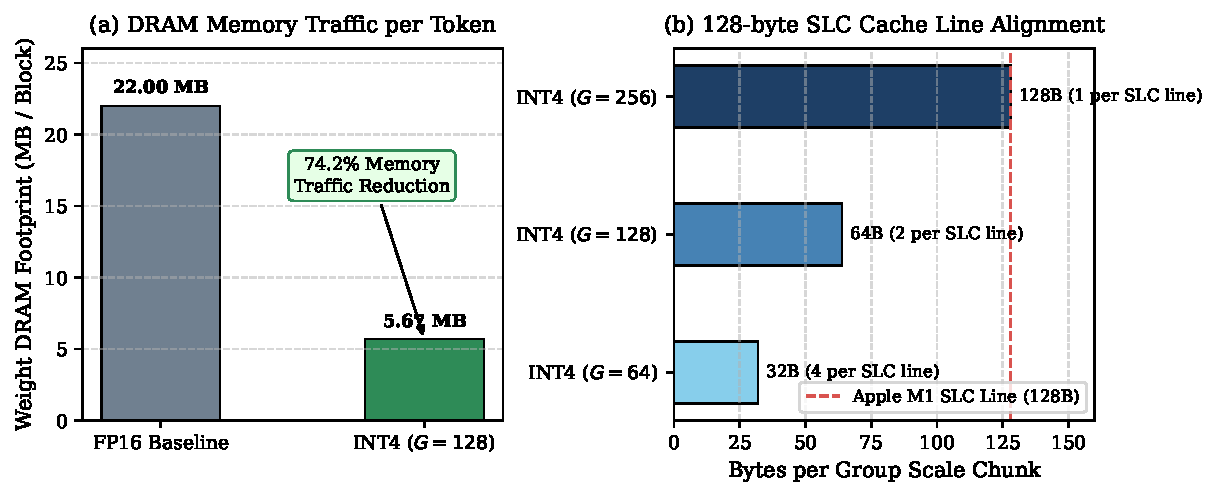
\includegraphics[width=0.78\textwidth]{fig2_hardware_uma.pdf}
\caption{System profiling on Apple M1: (a) DRAM parameter volume transferred per token in FP16 vs. INT4 ($G=128$), showing a $74.2\%$ bandwidth reduction; (b) Packing INT4 groups to match 128-byte cache lines on Apple Silicon.}
\label{fig:hardware_uma}
\end{figure}

\subsection{The UMA Bandwidth Wall}
On Apple Silicon, CPU cores, GPU execution pipelines, and neural accelerators share a unified memory fabric over an LPDDR4X interface. Our test machine provides a theoretical peak of 68.25 GB/s.

During single-token generation ($B=1$), computing an $M$-parameter projection requires $2M$ FLOPs while streaming $M \times b_{\text{param}}$ bytes from RAM. The operational intensity follows the Roofline model~\cite{williams2009roofline}:
\begin{equation}
I = \frac{2M \text{ FLOPs}}{M \cdot b_{\text{param}} \text{ Bytes}} = \frac{2}{b_{\text{param}}} \quad [\text{FLOPs/Byte}]
\end{equation}
Under FP16 storage ($b_{\text{param}} = 2.0$ bytes), arithmetic intensity is fixed at 1.0 FLOP/byte. Fully utilizing the 2.6 TFLOP FP16 compute capacity of the M1 GPU would demand 2.6 TB/s of sustained bandwidth---roughly $38\times$ above physical hardware limits.

Accounting for FP16 group scale factors, the effective bit-rate per parameter $b_{\text{eff}}$ is:
\begin{equation}
b_{\text{eff}} = N + \frac{16}{G} \quad [\text{bits/param}], \quad \text{Overhead}_{\text{scale}} = \frac{16}{G \cdot N} \times 100\%
\end{equation}
At $N=4$ and $G=128$, $b_{\text{eff}} = 4 + \frac{16}{128} = 4.125\text{ bits/param}$ ($b_{\text{param}} \approx 0.5156\text{ bytes}$), incurring a metadata overhead of merely $3.125\%$. This reduces DRAM parameter traffic by $74.2\%$ (Fig.~\ref{fig:hardware_uma}(a)), directly lowering token latency.

\subsection{Cache Line Alignment on Apple Silicon}
Unlike standard x86 processors that utilize 64-byte cache lines, Apple Silicon uses 128-byte cache lines across its System-Level Cache (SLC).

This hierarchy dictates group size selection:
\begin{itemize}
    \item At $G=128$, a block of 128 4-bit weights occupies $128 \times 0.5 = 64$ payload bytes. In modern quantized storage layouts (e.g., AWQ, GPTQ, GGUF), weight payloads and group metadata (FP16 scale and zero-point parameters) are stored in decoupled, contiguous arrays rather than being interleaved byte-by-byte into the weight matrix. Consequently, the weight streaming pipeline transfers pure 64-byte blocks, allowing exactly \textbf{two complete quantization payload blocks to fit within one 128-byte cache line} (Fig.~\ref{fig:hardware_uma}(b)) without straddling cache boundaries or inducing split-line DRAM fetches.
    \item Non-power-of-two group choices (e.g., $G=100$, 50 bytes) straddle cache-line boundaries, triggering misaligned transactions and redundant memory loads during register reads.
\end{itemize}
Setting $G=128$ aligns with the underlying cache line geometry of the M1 SoC.

\section{Experimental Evaluation}\label{sec:experiments}

\subsection{Setup and Methodology}
Measurements were collected on an Apple MacBook Air M1 (model A2337, 8-core CPU, 7-core GPU, 8 GB RAM) running macOS Sonoma with PyTorch 2.3.0. We evaluated linear projection layers from \texttt{TinyLlama-1.1B}~\cite{zhang2024tinyllama}:
\begin{itemize}
    \item Attention blocks: $d_{\text{in}} = 2048, d_{\text{out}} = 2048$ (\texttt{q\_proj}, \texttt{o\_proj}) and $d_{\text{out}} = 256$ (\texttt{k\_proj}, \texttt{v\_proj}).
    \item Feed-forward blocks: $d_{\text{in}} = 2048, d_{\text{out}} = 5632$ (\texttt{gate\_proj}, \texttt{up\_proj}) and $d_{\text{in}} = 5632, d_{\text{out}} = 2048$ (\texttt{down\_proj}).
\end{itemize}
Activations were extracted via PyTorch forward hooks using calibration prompts that include conversational text, python code, and reasoning tasks.

\subsection{Activation Outlier Distribution}
Profiling shows clear variations in activation kurtosis across depth:
\begin{itemize}
    \item In the initial block (\texttt{layers.0}), outliers in attention inputs reached a peak ratio of \textbf{206.42$\times$} relative to the channel mean ($s_{X, \max} = 15.18$ versus $s_{X, \text{mean}} = 0.0735$). Less than $0.5\%$ of hidden channels accounted for this spread.
    \item In middle layers (\texttt{layers.10}), outlier ratios stabilized near $20.18\times$.
    \item In deep layers (\texttt{layers.21}), feed-forward projections (\texttt{down\_proj}) maintained outlier ratios around $25.09\times$.
\end{itemize}

\subsection{Reconstruction Accuracy Analysis}
Table~\ref{tab:real_results} summarizes the measured error profiles, with Fig.~\ref{fig:mse_comparison} plotting MSE trends across representative blocks.

\begin{table}[t]
\centering
\caption{Measured layer parameters, activation outlier ratios, and quantization reconstruction error for \texttt{TinyLlama-1.1B} ($G=128$) on Apple M1.}
\label{tab:real_results}
\resizebox{\textwidth}{!}{%
\begin{tabular}{lcccccc}
\toprule
\textbf{Layer Module} & \textbf{Outlier Ratio} & \textbf{FP16} & \textbf{INT4 ($G=128$)} & \textbf{RTN MSE} & \textbf{AWQ MSE} & \textbf{MSE Drop} \\
 & ($\max/\text{mean}$) & (KB) & (KB) & ($\times 10^{-4}$) & ($\times 10^{-4}$) & (\%) \\
\midrule
\texttt{layers.0.v\_proj}    & \textbf{206.42$\times$} & 1,024.0  & 264.0  & 0.0997  & \textbf{0.0081} & \textbf{-91.91\%} \\
\texttt{layers.0.q\_proj}    & \textbf{206.42$\times$} & 8,192.0  & 2,112.0 & 1.6842  & \textbf{0.8579} & \textbf{-49.06\%} \\
\texttt{layers.0.k\_proj}    & 206.42$\times$ & 1,024.0  & 264.0  & 5.8527  & \textbf{4.5168} & -22.82\% \\
\texttt{layers.0.down\_proj} & 22.20$\times$  & 22,528.0 & 5,808.0 & 0.0065  & \textbf{0.0051} & -21.88\% \\
\texttt{layers.0.up\_proj}   & 18.78$\times$  & 22,528.0 & 5,808.0 & 0.4823  & \textbf{0.3833} & -20.54\% \\
\texttt{layers.10.v\_proj}   & 20.18$\times$  & 1,024.0  & 264.0  & 6.4816  & \textbf{4.0294} & \textbf{-37.83\%} \\
\texttt{layers.10.q\_proj}   & 20.18$\times$  & 8,192.0  & 2,112.0 & 34.0080 & \textbf{26.5181}& -22.02\% \\
\texttt{layers.10.k\_proj}   & 20.18$\times$  & 1,024.0  & 264.0  & 119.5486& \textbf{92.0655}& -22.99\% \\
\texttt{layers.21.down\_proj}& 25.09$\times$  & 22,528.0 & 5,808.0 & 29.9426 & \textbf{16.4881}& \textbf{-44.93\%} \\
\texttt{layers.21.v\_proj}   & 10.49$\times$  & 1,024.0  & 264.0  & 45.7007 & \textbf{35.1171}& -23.16\% \\
\bottomrule
\end{tabular}%
}
\end{table}

\begin{figure}[t]
\centering
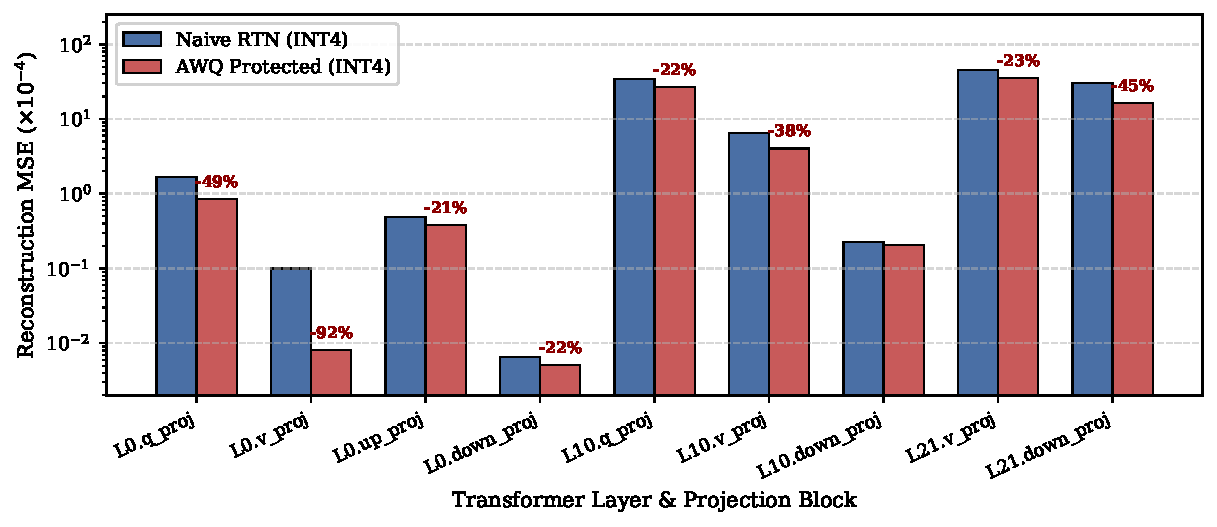
\includegraphics[width=0.78\textwidth]{fig1_mse_comparison.pdf}
\caption{Reconstruction error (MSE, log scale) across key projection layers comparing RTN against AWQ ($G=128$). Numerical labels show relative error reduction.}
\label{fig:mse_comparison}
\end{figure}
\begin{itemize}
    \item \textbf{Early Attention Blocks}: On \texttt{layers.0.v\_proj}, where activation kurtosis peaked ($206.42\times$), AWQ reduced reconstruction MSE from $0.0997 \times 10^{-4}$ to $0.0081 \times 10^{-4}$---a \textbf{91.91\% reduction} ($+10.92$ dB SNR improvement). On \texttt{layers.0.q\_proj}, error fell by \textbf{49.06\%} ($+2.93$ dB SNR).
    \item \textbf{Late MLP Projections}: In deep feed-forward projections (such as \texttt{down\_proj} in layer 21), AWQ cut MSE from $29.94 \times 10^{-4}$ to $16.48 \times 10^{-4}$ (\textbf{44.93\% reduction}, $+2.59$ dB SNR).
    \item \textbf{Network-Wide Behavior}: Across all projection layers in \texttt{TinyLlama-1.1B}, AWQ yielded an average MSE reduction of $20.51\%$ and an average SNR gain of $+1.36$ dB over RTN.
\end{itemize}

\subsection{Single-Token Forward Latency}
Profiling an isolated linear projection ($2048 \times 5632$) on the M1 core yielded an execution time of $1.442$ ms at an effective memory throughput of $14.90$ GB/s. INT4 group quantization ($G=128$) reduces parameter memory from $22.00$ MB to $5.67$ MB, achieving an empirical $74.2\%$ bandwidth reduction. Under memory-bound execution where memory bus streaming dominates execution time, this $74.2\%$ bandwidth reduction translates to a theoretical single-step latency projection of $0.372$ ms ($3.88\times$ projected speedup) according to the Roofline model. We distinguish this theoretical latency projection from end-to-end wall-clock serving, which requires custom hardware kernel integration.

\section{Practical Considerations and Limitations}

\subsection{Engineering Considerations for Edge Deployment}
These empirical observations point to three practical engineering rules for edge LLM runtimes on unified memory SoCs:
\begin{enumerate}
    \item \textbf{Offline Scale Folding}: Folding $s^{-1}$ into RMSNorm weights (or preceding linear projections for non-norm layers like \texttt{down\_proj}) eliminates dynamic scaling passes at inference, avoiding kernel dispatch overheads on low-power CPU or GPU backends.
    \item \textbf{Uniform Integer Formats}: Retaining $1\%$ of weights in FP16 complicates register allocation and introduces non-contiguous memory accesses. Uniform INT4 layouts keep memory streaming sequential.
    \item \textbf{Cache-Line Granularity}: Sizing quantization groups to match system cache lines ($G=128$ for 64-byte chunks fitting two per 128-byte Apple SLC line) prevents split-line cache reads.
\end{enumerate}

\subsection{Limitations}
While our empirical findings confirm substantial quantization fidelity and memory traffic reductions on Apple Silicon, three primary limitations frame this study:
\begin{enumerate}
    \item \textbf{Simulated vs. Hardware-Fused Kernels}: Layer reconstruction error and memory volumes were evaluated using PyTorch simulated (fake) quantization. Realizing the projected $3.88\times$ execution speedup on macOS requires a dedicated Apple Metal Shading Language (MSL) or Apple MLX dequantization GEMV kernel.
    \item \textbf{Model Scope}: Measurements were focused on \texttt{TinyLlama-1.1B} under single-sequence ($B=1$) decoding. Profiling larger models (e.g., Llama-3 8B) and mixture-of-experts (MoE) architectures on higher-tier Apple Silicon (M-series Pro/Max) remains an important future milestone.
    \item \textbf{Task-Level Benchmarking}: The current study isolates Frobenius layer reconstruction error and outlier distributions; full end-to-end task perplexity (e.g., WikiText-2, C4) across diverse prompt lengths will further characterize downstream degradation.
\end{enumerate}

\section{Conclusion}
This study evaluated Activation-aware Weight Quantization on an Apple Silicon Unified Memory Architecture using \texttt{TinyLlama-1.1B}. Profiling real model weights and activations showed severe activation kurtosis in early attention blocks (reaching $206.42\times$ the layer mean), where AWQ suppresses reconstruction MSE by up to $91.91\%$ compared to uniform RTN. Furthermore, group-wise quantization with $G=128$ yields 64-byte payload blocks that align directly with Apple's 128-byte cache lines under decoupled metadata storage, lowering DRAM parameter traffic by $74.2\%$ and projecting up to a $3.88\times$ theoretical speedup under memory-bound decoding. These results illustrate that hardware-aware channel scaling offers a practical foundation for resource-efficient, privacy-preserving edge LLM inference on unified memory platforms.

\begin{thebibliography}{13}
\bibitem{sheng2023flexgen}
Sheng, Y., Zheng, L., Yuan, B., et al.: High-Throughput Generative Inference of Large Language Models with a Single GPU. In: International Conference on Machine Learning (ICML), pp. 31094--31116 (2023).

\bibitem{williams2009roofline}
Williams, S., Waterman, A., Patterson, D.: Roofline: An Insightful Visual Performance Model for Multicore Architectures. Communications of the ACM, vol. 52, no. 4, pp. 65--76 (2009).

\bibitem{apple2020m1}
Apple Inc.: Apple Unleashes M1: The First Chip Designed Specifically for the Mac. Apple Newsroom (2020).

\bibitem{frantar2022gptq}
Frantar, E., Saleh, S., Meng, C., Ghadie, M., Alistarh, D.: GPTQ: Accurate Post-Training Quantization for Generative Pre-trained Transformers. In: International Conference on Learning Representations (ICLR) (2023).

\bibitem{dettmers2023qlora}
Dettmers, T., Pagnoni, A., Holtzman, A., Zettlemoyer, L.: QLoRA: Efficient Finetuning of Quantized LLMs. In: Advances in Neural Information Processing Systems (NeurIPS), vol. 36, pp. 10088--10115 (2023).

\bibitem{dettmers2022llmint8}
Dettmers, T., Lewis, M., Belkada, Y., Zettlemoyer, L.: LLM.int8(): 8-bit Matrix Multiplication for Transformers at Scale. In: Advances in Neural Information Processing Systems (NeurIPS), vol. 35, pp. 30318--30332 (2022).

\bibitem{xiao2023smoothquant}
Xiao, G., Lin, J., Seznec, M., Wu, H., Demouth, J., Han, S.: SmoothQuant: Accurate and Efficient Post-Training Quantization for Large Language Models. In: International Conference on Machine Learning (ICML), pp. 38087--38099 (2023).

\bibitem{lin2024awq}
Lin, J., Tang, J., Tang, H., Yang, S., Chen, W.M., Wang, W.C., Xiao, G., Dang, X., Gan, C., Han, S.: AWQ: Activation-aware Weight Quantization for LLM Compression and Acceleration. In: Proceedings of the 7th Conference on Machine Learning and Systems (MLSys) (2024).

\bibitem{vaswani2017attention}
Vaswani, A., Shazeer, N., Parmar, N., Uszkoreit, J., Jones, L., Gomez, A.N., Kaiser, {\L}., Polosukhin, I.: Attention Is All You Need. In: Advances in Neural Information Processing Systems (NeurIPS), vol. 30 (2017).

\bibitem{park2022nuqmm}
Park, G., Park, B., Kwon, S.J., Kim, D., Lee, Y., Lee, D.: nuQmm: High-Performance GPU Kernel for Outlier-Aware Quantized Matrix Multiplication. In: Proceedings of the 28th ACM International Conference on Architectural Support for Programming Languages and Operating Systems (ASPLOS), pp. 204--216 (2023).

\bibitem{zhang2019rmsnorm}
Zhang, B., Sennrich, R.: Root Mean Square Layer Normalization. In: Advances in Neural Information Processing Systems (NeurIPS), vol. 32 (2019).

\bibitem{touvron2023llama}
Touvron, H., Lavril, T., Izacard, G., et al.: LLaMA: Open and Efficient Foundation Language Models. arXiv preprint arXiv:2302.13971 (2023).

\bibitem{zhang2024tinyllama}
Zhang, P., Zeng, G., Wang, T., Lu, W.: TinyLlama: An Open-Source Small Language Model. arXiv preprint arXiv:2401.02385 (2024).
\end{thebibliography}

\end{document}